\documentclass[aps,prx,twocolumn,floatfix,nofootinbib,superscriptaddress]{revtex4-2}

\usepackage{amsmath,amssymb,bm}
\usepackage{booktabs,tabularx,array}
\usepackage{graphicx}
\usepackage{microtype}
\usepackage[colorlinks=true,linkcolor=blue,urlcolor=blue,citecolor=blue]{hyperref}

\newcolumntype{Y}{>{\raggedright\arraybackslash}X}
\newcommand{\code}[1]{\texttt{#1}}
\newcommand{\status}[1]{\textbf{#1}}
\setlength{\emergencystretch}{2em}

\begin{document}

\title{Streamlined Numerical Working Note and Experiment Plan}
\author{Asadullah Bhuiyan}
\affiliation{Department of Physics, Cornell University, Ithaca, New York 14853, USA}
\date{September 10, 2026}

\begin{abstract}
This living note is an analysis-first numerical plan for the adaptive class-A
fermion-circuit paper.  It replaces the assumption that every claim must be
regenerated on one new master ensemble.  The repository already contains strong
exact and stochastic evidence for bulk topology, a critical wall state, a
wall-localized slow tangent sector, wall-localized purification, and modular
packet handedness.  The immediate task is to analyze those data consistently
and run only the experiments needed to close a retained paper claim.  New Colab
work uses deterministic tasks, visible \code{tqdm} progress, completion-based
resume, and one rolling scientific checkpoint only for unusually long tasks.
The current modular-handedness extension is a local CPU campaign rather than a
Colab campaign.
\end{abstract}

\maketitle

\section{Purpose and working rules}

This is the single working experiment note to update as the paper scope changes.
It separates three questions:
\begin{enumerate}
\item What do the saved arrays already establish?
\item What analysis is missing although the simulation is complete?
\item What new simulation is required by the final manuscript claim?
\end{enumerate}

The default rule is \emph{analyze before rerunning}.  A legacy result is not
accepted merely because a figure exists, but an auditable raw archive is not
discarded because it predates the latest runner.  Protocol, geometry,
initialization, schedule, estimator, fit window, and source version must be
recorded.  A small same-seed equivalence test is preferred over a full rerun
when the only concern is engine provenance.

Exact Hamiltonian, mean-channel, stochastic Born-trajectory, postselected, and
modular-flow results remain separately labelled.  They may serve as calibration
or controls but are not pooled as measurements of the same object.

\section{Existing evidence and next actions}

\begin{table*}[t]
\caption{Initial evidence map.  The last column gives the smallest responsible
next action rather than a new master campaign.}
\label{tab:evidence}
\footnotesize
\renewcommand{\arraystretch}{1.15}
\begin{tabularx}{\textwidth}{@{}p{0.15\textwidth}p{0.25\textwidth}Yp{0.22\textwidth}@{}}
\toprule
Object & Existing evidence & Safe present claim & Next action \\
\midrule
Exact wall benchmark
& Twenty-two audited geometries; $c\simeq1$, correlator exponent near $2.074$,
opposite physical and modular velocities, and integer twist flow
& The target is a chiral $c=1$ free-fermion wall, with accepted $N_x=20$
& Reuse as calibration; do not rerun \\

Bulk stochastic topology
& Frozen production has 48 cases, 240 archives, and 1200 complex128
trajectories with topological and trivial controls.  The newer every-cycle
uniform campaign adds a balanced 1800-trajectory grid at $L=12$--$32$ for
$n_{\rm shell}=1,2,\mathrm{dense}$
& The tested adaptive circuit prepares the intended bulk phases
& Bulk validation is complete; do not run redesigned P1 or the retired
$L=36,40$ top-up \\

Wall-state CFT data
& Existing $S=100$ entropy/correlator data and a separate $S=10$ archive with
entropy, charge fluctuations, correlations, Chern data, tangent modes, and
records on the same trajectories
& The tested wall is consistent with $c\approx k\approx1$ and algebraic
correlations
& Formally analyze the joint $S=10$ archive before choosing a top-up \\

Tangent sector
& CPU and GPU campaigns show a small wall gap, a much larger trivial gap, and
approximately $96$--$97\%$ wall-plus-neighbour weight
& A finite-size slow tangent sector is strongly wall localized
& Extend only if a thermodynamic zero-gap claim remains \\

Purification
& $S=100$ max-mixed trajectories; approximately $93$--$94\%$ of the late
residual entropy lies on wall columns
& Purification is fast in the bulk and leaves a wall-localized residual
& Reanalyze completed width data; do not rerun a broad matrix \\

Chiral packet motion
& Legacy packets and recovered endpoint archives show opposite wall
displacements; hard topological has 20 trajectories and hard trivial has 25
& Modular packet transport is handed and absent in the matched-trivial control
& Resolve absolute sign; run the launched fixed-geometry CPU ensemble \\

Exact flux and mean channel
& Stable exact twist/pump calculations and a completed mean-channel matrix
& Exact and unconditional controls have oriented wall response
& Reuse as supplemental calibration, not sampled Born response \\
\bottomrule
\end{tabularx}
\end{table*}

The starting artifacts are the exact B0 audit, frozen P1 production, the
joint-observable $S=10$ archive, recovered endpoint archives, legacy Lyapunov
and purification campaigns, and the mean-channel production matrix.  Their
locations are catalogued in \path{PROJECT_ADMIN/DATA_CATALOG.md} and the
legacy evidence atlas.  This note should cite exact paths as each analysis is
completed rather than duplicating a second data catalog.

\section{Immediate analysis queue: no new GPU time}

\subsection{A0: uniform bulk-validation closure}

On September 9, 2026, the uniform perfect-correction validation campaign was
declared scientifically complete on its balanced $L=12,16,20,24,28,32$ grid.
For each size and $n_{\rm shell}=1,2,\mathrm{dense}$, the dataset contains
$S=100$ independent pure half-filled trajectories, no domain wall, 40
random-serial perfect-correction cycles, complex128 arithmetic, and the
trajectory-level real-space Chern and charge estimators at every cycle
including zero.  Thus the accepted comparison contains 18 cases and 1800
trajectories.  All 18 cycle-40 ensemble means lie between $0.99556$ and
$0.9999996$.

The planned completion of $L=36,40$ is retired.  Existing partial $L=36$
outputs remain preserved as supporting data but are excluded from the balanced
headline size series; no $L=40$ result is claimed.  The exact decision and data
boundary are recorded in
\path{experiment_review/uniform_bulk_validation_analysis/CAMPAIGN_CLOSURE.md}.

\subsection{A1: joint wall-state reduction}

Analyze the completed random-serial pure-state archive at $N_x=20$ and
$N_y=20,30,40,50$.  Use per-trajectory estimators followed by equal-weight
trajectory averaging.  Report:
\begin{enumerate}
\item entropy and charge-fluctuation slopes on identical interval windows;
\item $c$ and $k$ with trajectory-bootstrap intervals;
\item explicit-interface versus support-terminated construction differences;
\item matched-trivial null results;
\item fit-window and late-time sensitivity;
\item Chern, stationarity, and numerical-quality diagnostics.
\end{enumerate}
Only after A1 may a specific size or window be selected for a top-up.

\subsubsection{Power-law scaling of the $x$-averaged correlator}

Here is the critical prediction.  A chiral complex fermion has
$G(r_y)\sim d_{N_y}(r_y)^{-1}$, so the squared correlator measured in the
circuit must fall with exponent two,
\begin{equation}
 \begin{aligned}
 d_{N_y}(r_y)&=\frac{N_y}{\pi}
 \sin\!\left(\frac{\pi r_y}{N_y}\right),\\
 C_G(r_y)&\sim d_{N_y}(r_y)^{-\beta},
 \qquad \beta_{\rm crit}=2.
 \end{aligned}
 \label{eq:wall-correlator-critical-prediction}
\end{equation}
That is the number we want to see emerge; it is not imposed by the fit.

For trajectory $\xi$, first form the fixed-$x$ squared Green function
\begin{equation}
 C_{G,\xi}(x,r_y)=\frac{1}{2N_y}\sum_{y,\mu,\nu}
 \left|C_{\xi;(x,y,\mu),(x,y+r_y,\nu)}\right|^2,
 \label{eq:working-fixed-x-correlator}
\end{equation}
and then average across the transverse direction,
\begin{equation}
 C^{x\mathrm{av}}_{G,\xi}(r_y)=\frac{1}{N_x}
 \sum_x C_{G,\xi}(x,r_y).
 \label{eq:working-xavg-correlator}
\end{equation}
The $x$ average mixes the two algebraic wall pieces with short-ranged bulk
pieces.  The bulk contribution falls away quickly, leaving the wall power law
at the distances used here.  We fit each trajectory on
$2\le r_y\le\lfloor N_y/4\rfloor$, then summarize the resulting $\beta_\xi$
across the $S=100$ trajectories.

Figure~\ref{fig:working-correlator-scaling}(a) is the direct test: all six
circumferences follow the same algebraic envelope, close to the $d^{-2}$
prediction.  Panel (b) asks the finite-size question in the same form used
elsewhere in this note.  The measured exponent drifts from roughly $2.29$ at
the smaller circumferences to $2.23$ at the largest.  Extrapolations linear in
$1/N_y$ and $1/N_y^2$ land at $2.18$ and $2.23$, respectively.  The important
result is therefore simple: the stochastic wall has the predicted algebraic
sector and is moving toward two, while the remaining drift is still large
enough that we should call this consistency with $\beta=2$, not a precision
measurement of the thermodynamic exponent.

\begin{figure}[t]
\centering
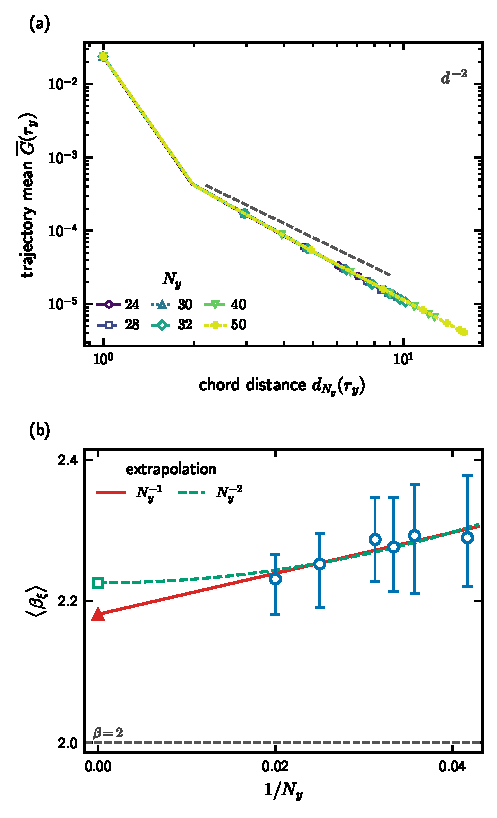
\includegraphics[width=\columnwidth]{domain_wall_correlator_scaling_analysis/outputs/hard_wall_finite_size_power_law.pdf}
\caption{\label{fig:working-correlator-scaling}Hard-wall correlator scaling at
$N_x=20$.  (a) Trajectory- and $x$-averaged squared correlator after $2N_y$
perfect-correction cycles; the dashed segment shows the critical $d^{-2}$
prediction.  (b) Mean trajectory exponent versus inverse circumference.  Each
size contains $S=100$ independent pure half-filled trajectories.  Fits use
$2\le r_y\le\lfloor N_y/4\rfloor$; bars show the trajectory interquartile
range.}
\end{figure}

The $x$-resolved archives let us make the sharper test directly on the two
programmed wall columns.  Repeating exactly the same fit at $x_L=5$ and
$x_R=15$ gives $\beta_L=2.17$--$2.18$ and $\beta_R=2.27$--$2.28$ across
$N_y=24,28,32$.  Averaging the two wall curves within each trajectory gives
$\beta_{\rm wall}=2.216$--$2.223$.  These values barely move with circumference
and the wall average lies closer to two than the full-$x$ average.  This is the
cleaner statement: the algebraic contribution is carried by the walls, while
the full-$x$ estimator retains a short-distance bulk admixture.  The persistent
left--right offset is visible rather than averaged away.  Since only three
circumferences retain the full $x$ resolution, we do not extrapolate them.

\begin{figure}[t]
\centering
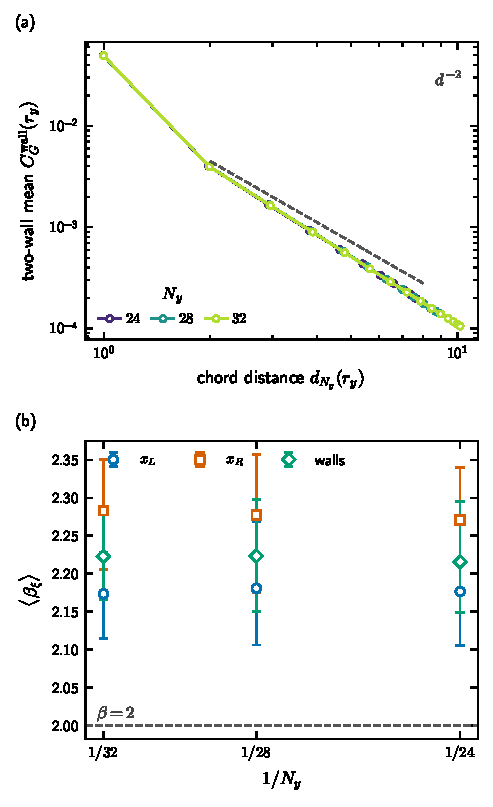
\includegraphics[width=\columnwidth]{domain_wall_correlator_scaling_analysis/outputs/hard_wall_xresolved_finite_size_power_law.pdf}
\caption{\label{fig:working-wall-resolved-scaling}Wall-resolved version of
Fig.~\ref{fig:working-correlator-scaling}.  (a) Mean of the $x_L$ and $x_R$
correlators, with the critical $d^{-2}$ guide.  (b) Exponents at each wall and
for their within-trajectory average.  Each size contains $S=100$ independent
pure half-filled trajectories evolved to $2N_y$ with hard-wall perfect
correction.  Fits use $2\le r_y\le\lfloor N_y/4\rfloor$; bars show the
trajectory interquartile range.}
\end{figure}

\subsection{A2: endpoint-packet reduction}

Combine only unique, verified endpoint slots.  Analyze hard and soft walls
separately.  For each wall report displacement, fitted velocity, fit quality,
packet retention, source/window sensitivity, and the matched-trivial result.

The circuit data move with wall 0 positive and wall 1 negative, whereas the
recent gate imported the opposite absolute orientation from the exact
benchmark.  This is a sign/protocol reconciliation problem, not an absence of
counterpropagation.  Tie wall labels to the circuit Chern and coordinate
conventions; do not silently flip the sign.  Treat poor soft-wall retention as
a separate reported limitation.

\subsection{A2b: launched fixed-geometry modular-handedness ensemble}

On September 3, 2026, a new trajectory-first CPU campaign was locked and
launched from
\path{00_WORKSPACE/CURRENT/modular_handedness_cpu_pilot/}.  It contains 100
independent hard-wall and 100 independent soft-wall trajectories at
$N_x=20$, $N_y=40$, $n_{\rm shell}=1$, with $80=2N_y$ physical cycles,
perfect correction, pure half filling, the legacy raster-$y$ order, and
complex128 arithmetic.  The hard construction is support truncated with
slab-only dynamics; the soft construction is the untruncated explicit
interface.  The root seed is \code{2026090302}.

Each deterministic task calls the canonical CPU
\code{classA\_U1FGTN.run\_markov\_circuit}, saves only its final occupied
frame, and publishes an NPZ/completion-JSON pair.  Modular reduction is a
separate resumable stage: all 40 translated half-cylinder cuts are constructed
and propagated within each trajectory before any ensemble average.  The
primary fit is a free-intercept fit on $1\le t_{\rm mod}\le5$, with locked
fit-window, spectral-cutoff, and wall-window sensitivity analyses.  Whole
trajectories are bootstrapped with 10,000 fixed-seed draws.

The production session is \code{modular\_handedness\_s100} on host
\code{jian1}, pinned to 28 physical cores on NUMA node 0.  Its stable output
root is
\path{modular_handedness_cpu_pilot/outputs/modular_handedness_nx20_ny40_hard_soft_s100_v1/}.
The simulation configuration hash is
\path{f9a49e33e4f8401a4fbea340272cfd5d9b1ca1f6e5ecdd3c1efd61ba04ea14b1};
the analysis configuration hash is
\path{c0042b1bcb3b9aa33b03fa7a8fe6498e2955d2cf470f47c9f68a4a5b4ec3d836}.
The measured completion estimate is 8--10 hours.  The absolute wall-Chern
orientation remains unresolved, so raw $+y$ velocities stay primary and no
post-hoc sign flip is permitted.

\subsection{A3: transverse-width purification audit}

Regenerate the conclusion from the completed $N_x=20,24,28$, $N_y=20$ max-mix
data.  Report wall and bulk purification times, late wall entropy, uncertainty,
and whether a transverse trend is resolved.  This is an analysis repair, not a
new simulation campaign.

\section{Minimal new simulation queue}

New work begins only after the corresponding analysis is complete, except for
the explicitly authorized A2b fixed-geometry campaign:
\begin{enumerate}
\item \status{H1 fixed-geometry ensemble:} the 100 hard plus 100 soft CPU
campaign in A2b is launched; resume the same stable output root if interrupted.
\item \status{Engine equivalence:} replay one small or moderate fixed-seed case
with the current canonical GPU engine and compare the scientific arrays at the
appropriate tolerance.
\item \status{Wall-state top-up:} after A1, select at most one or two geometries
targeted at the observed uncertainty or finite-size weakness.  Finishing the
incomplete $N_y=60$ archive is a candidate, not an automatic requirement.
\end{enumerate}

There is no current authorization for a fresh P1 campaign, continuation of the
retired $L=36,40$ uniform-bulk extension, broad purification rerun, or
additional large parameter scan beyond A2b.

\section{Claim-dependent optional work}

\begin{description}
\item[Thermodynamic tangent closing.]
Run more sizes and longer time convergence only if the paper claims a
thermodynamic zero tangent gap.  Otherwise retain the supported finite-size
statement.

\item[Higher-Renyi common ensemble.]
Measure $q=2,3$ entropies and charge fluctuations on a small common ensemble
only if precision CFT consistency is central.

\item[Frozen-record stochastic flux.]
Run a minimal fixed-record replay only if a branchwise integer index is needed.
Exact twist and pump results already provide calibration.

\item[True feedback or phase-noise robustness.]
Design a separate campaign only if a quantitative robustness interval becomes
a paper claim.  Partial postselection is not imperfect feedback.
\end{description}

\section{Deferred from the core plan}

The following are not prerequisites for the current central physics:
\begin{itemize}
\item full sampled Born modular-response susceptibility, whose score term is
currently noise dominated;
\item the 5500-trajectory log-Gram $\alpha$ scan;
\item many-body operator-CFT or record-CFT towers;
\item a universal same-record tangent--purification exponent;
\item large phase-noise and feedback-error matrices.
\end{itemize}
These may become separate projects but should not be presented as validation of
an otherwise unsupported wall state.

\section{Simple Colab execution contract}

Every new notebook follows the repository policy:
\begin{enumerate}
\item one notebook, one runner, the canonical GPU engine, and only required
observer modules;
\item code copied from Drive to local \path{/content} before execution;
\item deterministic configurations or immutable shards of at most five
trajectories;
\item an outer \code{tqdm} task bar and an inner cycle, trajectory, batch, or
scan-point bar;
\item local scratch and compact streamed observables;
\item one atomic result plus a completion JSON written last;
\item restart by checksum-verifying completed tasks;
\item for tasks longer than roughly one hour, one rolling checkpoint containing
native state, ranks, RNG states, observer accumulators, configuration identity,
and completed cycle or point.
\end{enumerate}

The default design excludes a second Drive API path, server leases,
generation/pointer protocols, remote-status subprocesses, migration ledgers,
session dashboards, and automatic orphan repair.  A Drive failure leaves the
task pending.  Rerunning continues from the last verified task or checkpoint.

\section{Working decision ledger}

\begin{table}[b]
\caption{Living decisions for the next revision.}
\label{tab:decisions}
\footnotesize
\renewcommand{\arraystretch}{1.12}
\begin{tabularx}{\columnwidth}{@{}p{0.28\columnwidth}Y@{}}
\toprule
Decision & Current position \\
\midrule
Bulk P1 & Complete; no rerun \\
Exact B0 & Complete; reuse \\
Wall CFT & Analyze existing joint archive first \\
H1 chirality & Packet handedness primary; S100 hard plus S100 soft CPU campaign launched; resolve absolute sign \\
Born response & Remove from core \\
Soft wall & Report retention limitation before further runs \\
Tangent & Keep finite-size claim unless more scaling is requested \\
Stochastic flux & Optional \\
Operator/record CFT & Deferred \\
Colab design & Simple task resume plus one rolling checkpoint for long tasks \\
\bottomrule
\end{tabularx}
\end{table}

\section{Open questions for the next update}

\begin{enumerate}
\item What is the shortest final statement of the paper's central numerical
claim?
\item Is consistency with $c=k=1$ sufficient, or is a precision
higher-Renyi/common-ensemble test required?
\item Is a finite-size localized tangent sector sufficient, or must the paper
claim a thermodynamic gap closing?
\item Does the paper require a stochastic branchwise integer flux invariant?
\item Should the soft-wall packet construction remain in the main text, move
to the supplement as a limitation, or be removed?
\end{enumerate}

\paragraph*{Revision rule.}
Future updates edit this document in place.  Completed analyses move into
Table~\ref{tab:evidence}; rejected ideas move to the deferred section with a
one-sentence reason; new experiments must name the paper claim they support.

\end{document}
